\section{HadoopDB}
Hadoop  представляет собой платформу для построения приложений, способных обрабатывать огромные объемы данных. 
Система основывается на распределенном подходе к вычислениям и хранению информации, основными ее особенностями являются:
\begin{itemize}
\item \textbf{Масштабируемость:} с помощью Hadoop возможно надежное хранение и обработка огромных объемов данных, 
которые могут измеряться петабайтами;
\item \textbf{Экономичность:} информация и вычисления распределяются по кластеру, построенному на самом 
обыкновенном оборудовании. Такой кластер может состоять из тысяч узлов;
\item \textbf{Эффективность:} распределение данных позволяет выполнять их обработку параллельно на множестве компьютеров, 
что существенно ускоряет этот процесс;
\item \textbf{Надежность:} при хранении данных возможно предоставление избыточности, благодаря хранению нескольких копий. 
Такой подход позволяет гарантировать отсутствие потерь информации в случае сбоев в работе системы;
\item \textbf{Кроссплатформенность:} так как основным языком программирования, используемым в этой системе является Java, 
развернуть ее можно на базе любой операционной системы, имеющей JVM.
\end{itemize}

\textbf{HDFS}

В основе всей системы лежит распределенная файловая система под незамысловатым названием Hadoop 
Distributed File System. Представляет она собой вполне стандартную распределенную файловую систему, но все же 
она обладает рядом особенностей:
\begin{itemize}
\item Устойчивость к сбоям, разработчики рассматривали сбои в оборудовании скорее как норму, чем как исключение;
\item Приспособленность к развертке на самом обыкновенном ненадежном оборудовании;
\item Предоставление высокоскоростного потокового доступа ко всем данным;
\item Настроена для работы с большими файлами и наборами файлов;
\item Простая модель работы с данными: один раз записали~--- много раз прочли;
\item Следование принципу: переместить вычисления проще, чем переместить данные;
\end{itemize}

\textbf{Архитектура HDFS}

\begin{figure}[ht!]
\center{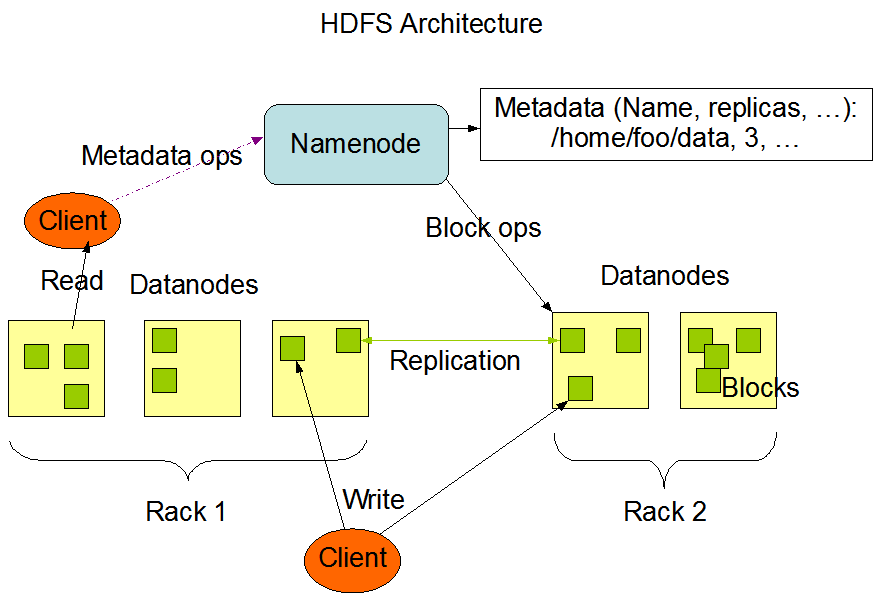
\includegraphics[width=1\textwidth]{hdfsarchitecture}}
\caption{Архитектура HDFS}
\label{ris:hdfsarchitecture}
\end{figure}

\begin{itemize}
\item \textbf{Namenode}

Этот компонент системы осуществляет всю работу с метаданными. Он должен быть запущен только на одном компьютере 
в кластере. Именно он управляет размещением информации и доступом ко всем данным, расположенным на ресурсах кластера. 
Сами данные проходят с остальных машин кластера к клиенту мимо него.

\item \textbf{Datanode}

На всех остальных компьютерах системы работает именно этот компонент. Он располагает сами блоки данных в локальной 
файловой системе для последующей передачи или обработки их по запросу клиента. Группы узлов данных принято называть 
Rack, они используются, например, в схемах репликации данных.

\item \textbf{Клиент}

Просто приложение или пользователь, работающий с файловой системой. В его роли может выступать практически что угодно.
\end{itemize}

Пространство имен HDFS имеет классическую иерархическую структуру: пользователи и приложения имеют возможность 
создавать директории и файлы. Файлы хранятся в виде блоков данных произвольной (но одинаковой, за исключением последнего; 
по-умолчанию 64 mb) длины, размещенных на Datanode'ах. Для обеспечения отказоустойчивости блоки хранятся в нескольких 
экземплярах на разных узлах, имеется возможность настройки количества копий и алгоритма их распределения по системе. 
Удаление файлов происходит не сразу, а через какое-то время после соответствующего запроса, так как после получения 
запроса файл перемещается в директорию /trash и хранится там определенный период времени на случай если пользователь 
или приложение передумают о своем решении. В этом случае информацию можно будет восстановить, в противном случае~--- физически удалить.

Для обнаружения возникновения каких-либо неисправностей, Datanode периодически отправляют Namenode'у сигналы о 
своей работоспособности. При прекращении получения таких сигналов от одного из узлов Namenode помечает его как <<мертвый>>, 
и прекращает какой-либо с ним взаимодействие до возвращения его работоспособности. Данные, хранившиеся на <<умершем>> узле 
реплицируются дополнительный раз из оставшихся «в живых» копий и система продолжает свое функционирование как ни в чем не бывало.

Все коммуникации между компонентами файловой системы проходят по специальным протоколам, основывающимся на стандартном TCP/IP. 
Клиенты работают с Namenode с помощью так называемого ClientProtocol, а передача данных происходит по DatanodeProtocol, 
оба они обернуты в Remote Procedure Call (RPC).

Система предоставляет несколько интерфейсов, среди которых командная оболочка DFSShell, набор ПО для администрирования DFSAdmin, 
а также простой, но эффективный веб-интерфейс. Помимо этого существуют несколько API для языков программирования: Java API, 
C pipeline, WebDAV и так далее.

\textbf{MapReduce}

Помимо файловой системы, Hadoop включает в себя framework для проведения масштабных вычислений, обрабатывающих 
огромные объемы данных. Каждое такое вычисление называется Job (задание) и состоит оно, как видно из названия, из двух этапов:

\begin{itemize}
\item \textbf{Map}

Целью этого этапа является представление произвольных данных (на практике чаще всего просто пары ключ-значение) в виде 
промежуточных пар ключ-значение. Результаты сортируются и групируются по ключу и передаются на следующий этап.

\item \textbf{Reduce}

Полученные после map значения используются для финального вычисления требуемых данных. Практические любые данные могут 
быть получены таким образом, все зависит от требований и функционала приложения.
\end{itemize}

Задания выполняются, подобно файловой системе, на всех машинах в кластере (чаще всего одних и тех же). Одна из них выполняет 
роль управления работой остальных — JobTracker, остальные же ее бесприкословно слушаются — TaskTracker. В задачи 
JobTracker'а входит составление расписания выполняемых работ, наблюдение за ходом выполнения, и перераспределение в случае 
возникновения сбоев.

В общем случае каждое приложение, работающее с этим framework'ом, предоставляет методы для осуществления этапов map и reduce, 
а также указывает расположения входных и выходных данных. После получения этих данных JobTracker распределяет задание между 
остальными машинами и предоставляет клиенту полную информацию о ходе работ.

Помимо основных вычислений могут выполняться вспомогательные процессы, такие как составление отчетов о ходе работы, кэширование, 
сортировка и так далее.

\textbf{HBase}

В рамках Hadoop доступна еще и система хранения данных, которую правда сложно назвать СУБД в традиционном смысле этого слова. 
Чаще проводят аналогии с проприетарной системой этого же плана от Google~--- BigTable.

HBase представляет собой распределенную систему хранения больших объемов данных. Подобно реляционным СУБД данные хранятся в 
виде таблиц, состоящих из строк и столбцов. И даже для доступа к ним предоставляется язык запросов HQL (как ни странно~--- 
Hadoop Query Language), отдаленно напоминающий более распространенный SQL. Помимо этого предоставляется итерирующмй интерфейс 
для сканирования наборов строк.

Одной из основных особенностей хранения данных в HBase является возможность наличия нескольких значений, 
соответствующих одной комбинации таблица-строка-столбец, для их различения используется информация о времени добавления записи. 
На концептуальном уровне таблицы обычно представляют как набор строк, но физически же они хранятся по столбцам, достаточно 
важный факт, который стоит учитывать при разработки схемы хранения данных. Пустые ячейки не отображаются каким-либо образом 
физически в хранимых данных, они просто отсутствуют. Существуют конечно и другие нюансы, но я постарался упомянуть лишь основные.

HQL очень прост по своей сути, если Вы уже знаете SQL, то для изучения его Вам понадобится лишь просмотреть по диагонали 
коротенький вывод команды help;, занимающий всего пару экранов в консоли. Все те же SELECT, INSERT, UPDATE, DROP и так далее, 
лишь со слегка измененным синтаксисом.

Помимо обычно командной оболочки HBase Shell, для работы с HBase также предоставлено несколько API для различных языков 
программирования: Java, Jython, REST и Thrift.

\textbf{HadoopDB}

В проекте HadoopDB специалисты из университетов Yale и Brown предпринимают попытку создать гибридную систему управления 
данными, сочетающую преимущества технологий и MapReduce, и параллельных СУБД. В их подходе MapReduce обеспечивает коммуникационную 
инфраструктуру, объединяющую произвольное число узлов, в которых выполняются экземпляры традиционной СУБД. Запросы формулируются 
на языке SQL, транслируются в среду MapReduce, и значительная часть работы передается в экземпляры СУБД. Наличие MapReduce 
обеспечивается масштабируемость и отказоустойчивость, а использование в узлах кластера СУБД позволяет добиться высокой 
производительности. 


\section{Установка и настройка}
Вся настройка ведется на Ubuntu Server операционной системе.

Перед тем, как приступить собственно говоря к установке Hadoop, необходимо выполнить два элементарных действия, 
необходимых для правильного функционирования системы:
\begin{itemize}
\item открыть доступ одному из пользователей по ssh к этому же компьютеру без пароля, 
можно например создать отдельного пользователя для этого [hadoop]:
\begin{verbatim}
sudo groupadd hadoop
sudo useradd -m -g hadoop -d /home/hadoop -s /bin/bash \
-c "Hadoop software owner" hadoop
\end{verbatim}

Далее действия выполняем от его имени:
\begin{verbatim}
su hadoop
\end{verbatim}

Генерируем RSA-ключ для обеспечения аутентификации в условиях отсутствия возможности использовать пароль:
\begin{verbatim}
hadoop@localhost ~ $ ssh-keygen -t rsa -P ""
Generating public/private rsa key pair.
Enter file in which to save the key (/home/hadoop/.ssh/id_rsa):
Your identification has been saved in /home/hadoop/.ssh/id_rsa.
Your public key has been saved in /home/hadoop/.ssh/id_rsa.pub.
The key fingerprint is:
7b:5c:cf:79:6b:93:d6:d6:8d:41:e3:a6:9d:04:f9:85 hadoop@localhost
\end{verbatim}

И добавляем его в список авторизованных ключей:
\begin{verbatim}
cat $HOME/.ssh/id_rsa.pub >> $HOME/.ssh/authorized_keys
\end{verbatim}

Этого должно быть более чем достаточно, проверить работоспособность соединения можно просто написав:
\begin{verbatim}
ssh localhost
\end{verbatim}

Не забываем предварительно инициализировать sshd:
\begin{verbatim}
/etc/init.d/sshd start
\end{verbatim}

\item Помимо этого необходимо убедиться в наличии установленной JVM версии 1.5.0 или выше.
\begin{verbatim}
sudo aptitude install openjdk-6-jdk
\end{verbatim}
\end{itemize}
